\documentclass[../main-v1.tex]{subfiles}
\begin{document}
\chapter{Code Management \hideme{comments from Anne /BV included 5/8}}
\label{ch:codemgmt}


%%%%%%%%%%%%%%%%%%%%%%%%%%%%%%%%
\section{Liquid Argon TPC Code Management \hideme{Junk/Calcutt - needs update}}
\label{sec:codemgmt:dunetpc}  %% fix label according to section

Software for simulation, data read-in, and reconstruction %shares significant 
has a great deal of commonality across the % anne
liquid-argon time projection chamber detectors 
 planned to be deployed by DUNE including prototypes.  These  
  include the %anne 
  horizontal- and vertical-drift far detector modules, the 35-ton prototype, ProtoDUNE-SP, ProtoDUNE-DP, ProtoDUNE-2-HD, ProtoDUNE-VD, ICEBERG, and the pixel \dword{nd} and its prototypes.
%the \dword{sphd} and \dword{spvd} \dwords{detmodule}, the \dword{35t}, \dword{pdsp}, \dword{pddp}, \dword{protodune2},  the pixel \dword{nd} and its prototypes. 
The same software stack used by \dword{dune} and the protoDUNE detectors is used for the wire readout, the photon detectors, and the cosmic-ray taggers  in some of the prototypes.  

Despite the commonalities, the interfaces to event generators, \dword{geant4}, \dword{art} and the data handling systems require effort to build and maintain, and data products need to be thought out carefully.  To reduce the development burden and expand the pool of expertise, DUNE has chosen to use the \dword{larsoft} toolkit, which is built on NuTools and \dword{art}.  

\dword{larsoft} itself is split up into several repositories, such as larcore, larsim, larevt, lardata, and variations that have been split from them over time, such as lardataobj.  \dword{larsoft} is supported by \dword{fnal}'s Scientific Computing Division (SCD) and is shared among several other experiments, such as ArgoNeuT, MicroBooNE, ICARUS and SBND. The pool of potential developers is quite large,  with a variety
 of software experience and length of time commitment to maintenance.
Substantial effort goes into maintaining coherence across the project with new releases of \dword{larsoft}   made weekly.  DUNE's \dword{larsoft}-based code stack follows a similar release schedule.


DUNE's \dword{larsoft}-based software historically had been collected in a single git repository called dunetpc, starting in the early days of the collaboration.  This repository was hosted using \dword{fnal}'s Redmine service.  Compiling all of the code in this single repository became slower as more source files were added.  In January 2022, a split of the dunetpc repository into ten smaller repositories was deployed on GitHub, taking advantage of GitHub's superior performance, feature set, and openness compared with Redmine.  The old dunetpc repository is kept in a read-only state in Redmine for inspection purposes.  The new top-level product is called dunesw.  A \dword{ups} dependency graph made in January 2022 is shown in Figure~\ref{fig:dunetpcdeptree}, showing the dunesw stack, the \dword{larsoft} \dword{ups} products, and their dependencies.

\begin{dunefigure}
[Dependency graph for the dunesw software stack, Jan 2022]
{fig:dunetpcdeptree}
{\dword{ups} dependency graph for the dunesw software stack, for version v09\_42\_00\_01, January 2022.}
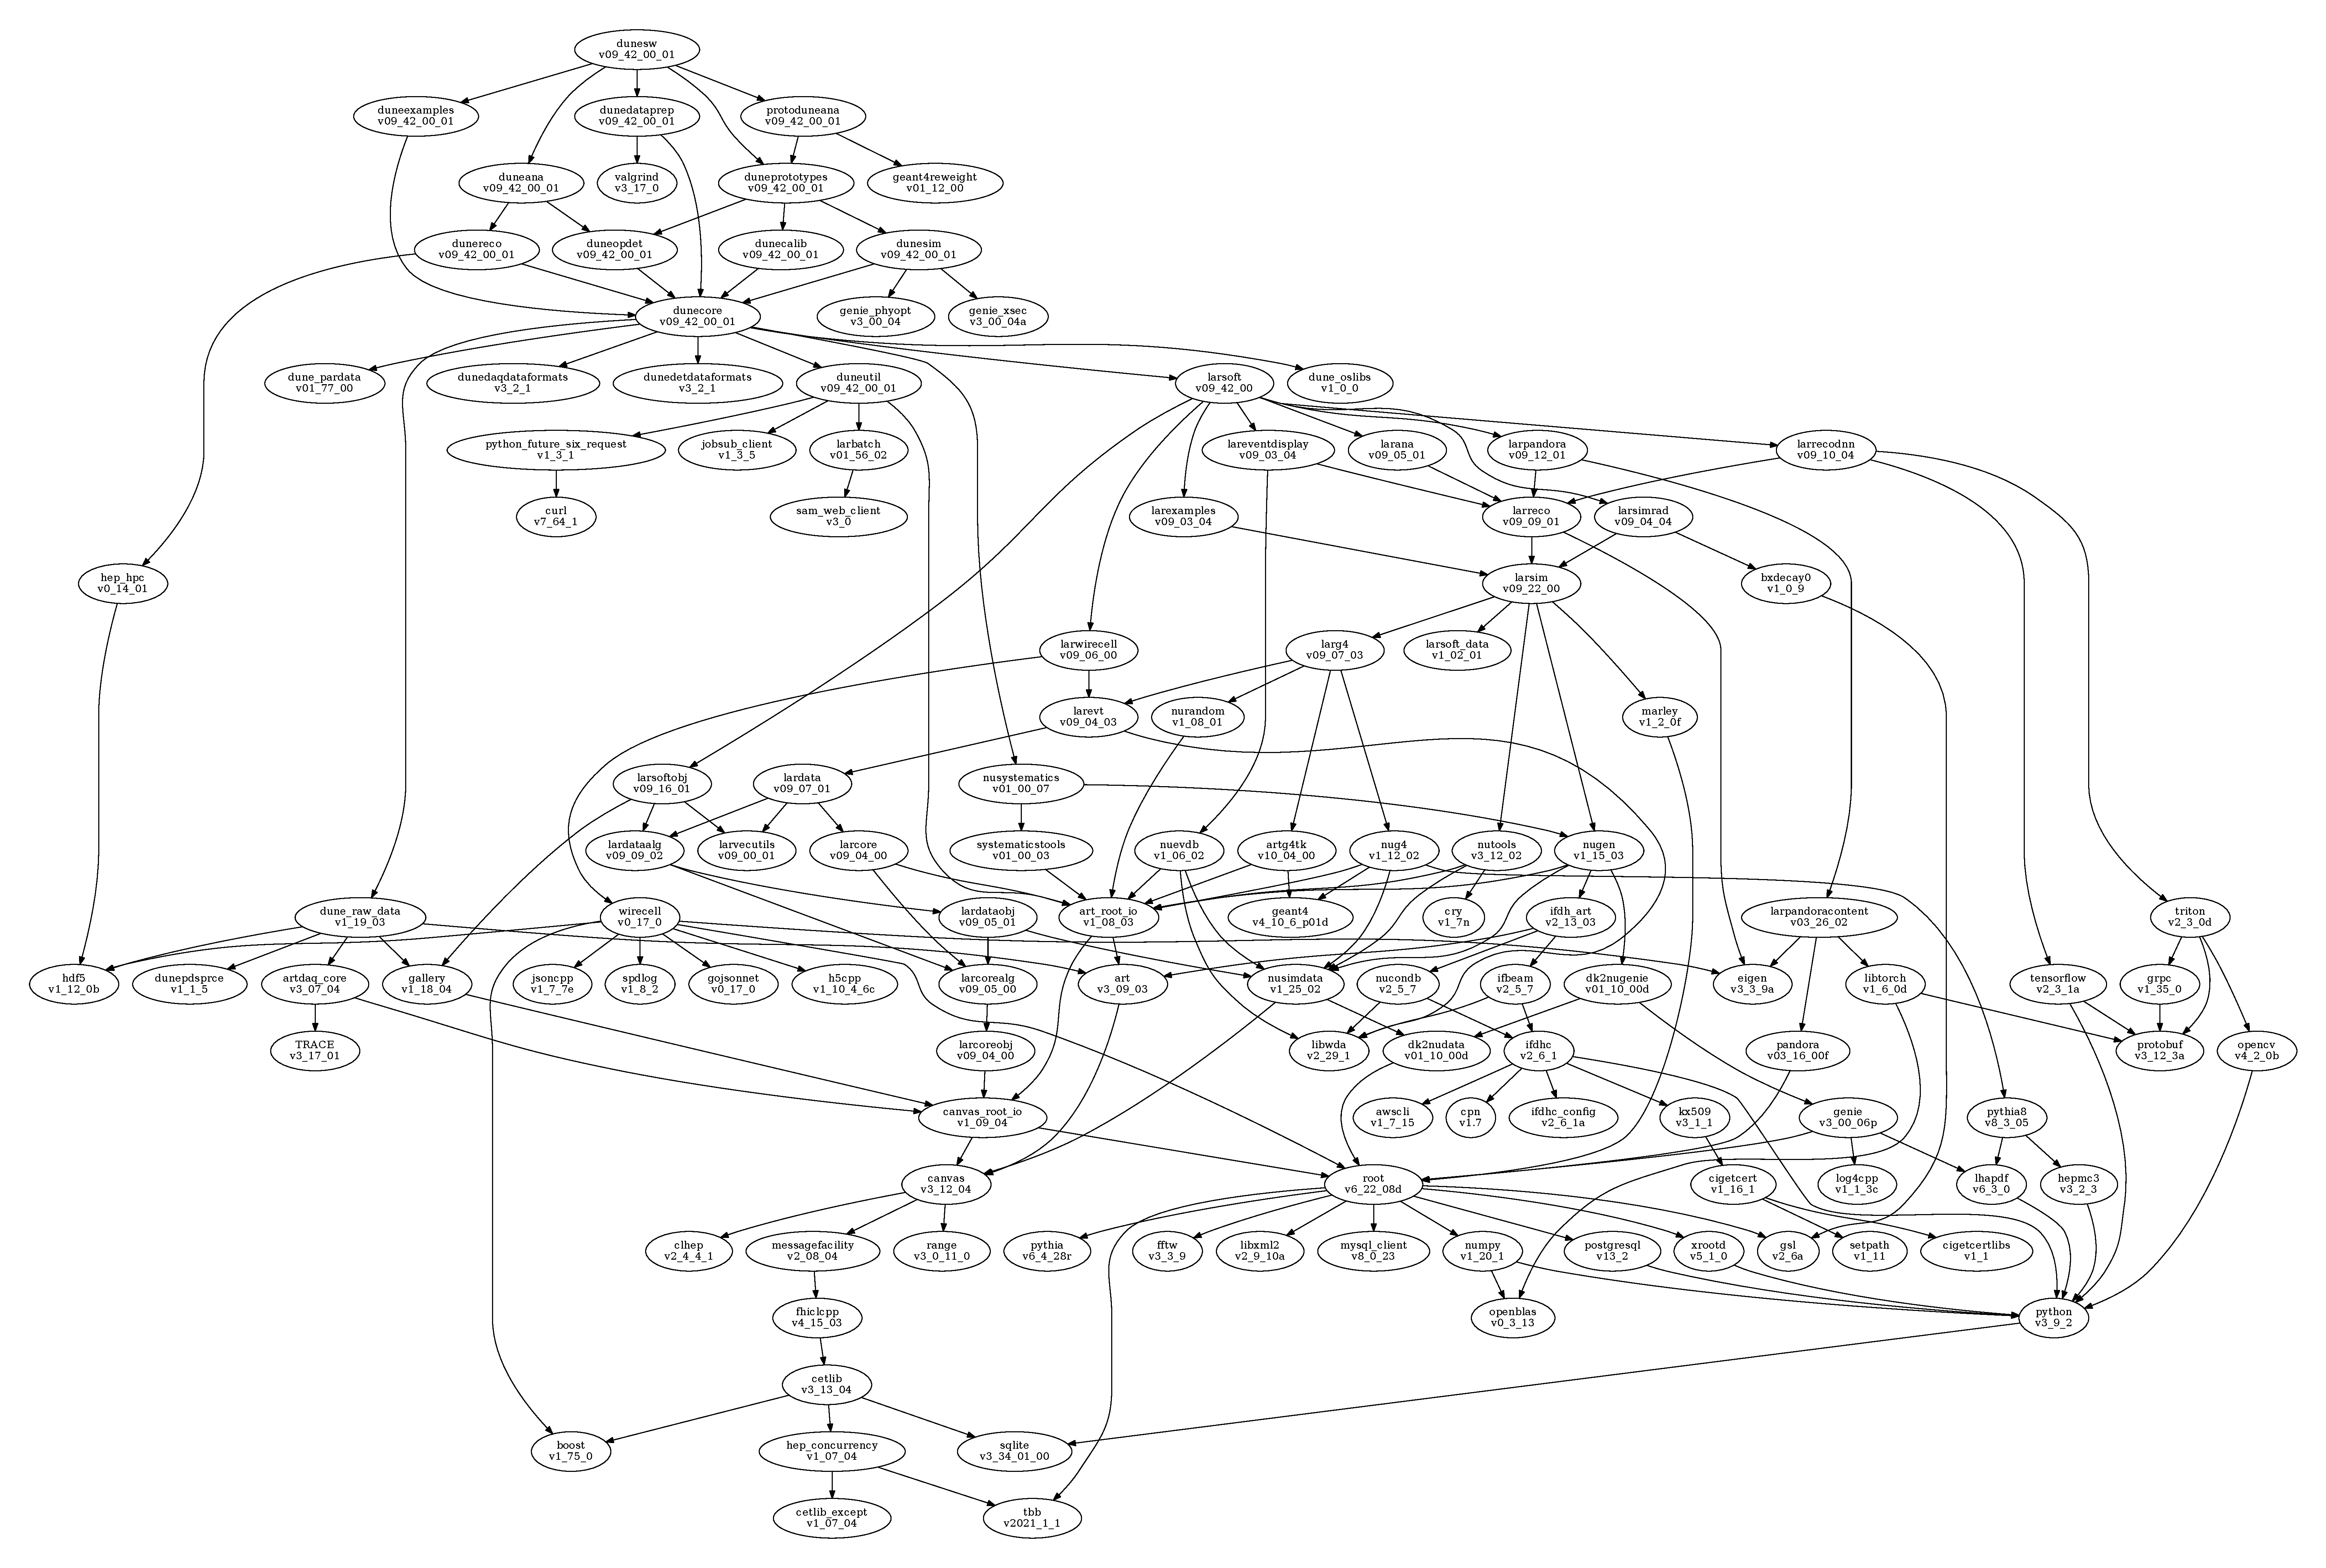
\includegraphics[width=\textwidth]{graphics/CodeManagementFigures/dunesw_v09_42_00_01_graph.pdf}
\end{dunefigure}

Since the dunesw stack depends on \dword{larsoft} and sets it up via \dword{ups}, dunesw also has a weekly release schedule, and releases are tied to \dword{larsoft}'s releases and use the same version tag names.  \dword{larsoft}'s repositories had been hosted in \dword{fnal}'s Redmine instance until 2018, at which point they were migrated to GitHub.  At the same time, a pull-request model was instituted.  \dword{larsoft}'s pull-request system, based on the one used by the CMS experiment, performs automated checks that the proposed new code compiles and tests properly.  Once the tests are successful, a review of the proposed new code is required before it can be merged into the repository.  As of this writing, DUNE is considering moving to a pull-request model similar to that of \dword{larsoft}.

The build system used is {\tt mrb}, which is provided by and supported by \dword{fnal}'s SCD.  Software is built in \dword{ups} products which are distributed to the collaboration in two ways.  The primary distribution mechanism is via a set of installed products in the \dword{cvmfs} which can be directly set up by end users of Scientific Linux 7 and CENTOS 8 without the need to install anything locally.  \dword{cvmfs} maintains a cache on the user's computer to store copies of the released software files for repeated local access.  \dword{cvmfs} is also used to distribute released software to batch worker nodes.  The second software distribution mechanism is via the {\tt scisoft.fnal.gov} web server.  When a release is made, the repositories are tagged and the release manager triggers \dword{fnal}'s Jenkins build servers to compile the software and install auxiliary files in \dword{ups} products.  The \dword{ups} products are then tarred up and the tarballs are uploaded to the scisoft web server, along with a manifest file that describes which tarballs need to be downloaded and installed to get a fully
functioning dunesw software stack.

In addition to code, some data files also are distributed via \dword{cvmfs}.  For example, photon lookup libraries are stored in several-hundred-megabyte rootfiles which are inconvenient to store in a git repository.  They are loaded into a special repository in \dword{cvmfs} and scisoft called {\tt dune\_pardata}.  Even larger files are stored in \dword{stashcache} which has a \dword{cvmfs} interface for the user, but which retrieves files out of a dedicated area in \dword{dcache}.

As operating systems have become more secure, some of the ways of distributing, setting up, and running HEP software, such as the use of the environment variables {\tt LD\_LIBRARY\_PATH} and {\tt DYLD\_LIBRARY\_PATH}, have conflicted with security features of at least one operating system.  We are evaluating \dword{spack} as a replacement for {\tt mrb} and \dword{ups}.  \dword{spack} is a build system that also allows users to select from a list of installed versions, like \dword{ups} does. \dword{ups} is now approximately 25 years old, it is not an industry standard, and it is somewhat linked to \dword{fnal}.  \dword{spack} has a significant community using it outside of HEP, and thus there is a large volume of documentation available for it on the web.  The DAQ group is already using \dword{spack} for online systems. 


%\fixme{(anne) the following seems like it's too much in the weeds for a CDR, no?}
%One of these % anne would add "conflicts" if we keep this 
%is the use of the symbol {\tt LD\_LIBRARY\_PATH}.  \dword{ups} uses {\tt LD\_LIBRARY\_PATH} to point a user's environment at directories that contain the versions of released products that can be loaded and run.  Changing the contents of the {\tt LD\_LIBRARY\_PATH} variable causes the same program to load different versions of libraries.  Proper use of \dword{ups} maintains compatibility.  However, with newer operating systems, the shared libraries that are linked with programs and other shared libraries must be in the same locations as they where when linked, and not relocated.  The library that links to another keeps track of the installed locations of the libraries it links with.  Alternatively, the paths in which the dependent libraries are found can be edited after installation, in effect re-performing a stage of the linking step.  Spack is aware of this and inserts the proper {\tt rpath} values into linked libraries.

%repeat The use of Spack is under evaluation.  %anne moved up \dword{ups} is now approximately 25 years old and it is not an industry standard, and it is somewhat linked to \dword{fnal}.  Spack has a significant community using it outside of HEP, and thus there is a large volume of documentation available for it on the web.

%%%%%%%%%%%%%%%%%%%%%%%%%%%%%%%%
\section{Near Detector Code Management \hideme{Muether/Cremonisi/Junk needs update}}
\label{sec:codemgmt:neardet}  %% fix label according to section

%The \dword{nd} consists of three components.  
When DUNE starts running with beam, the expected \dword{nd} configuration will consist of a \dword{lartpc} with pixel readout (\dword{ndlar}), a magnetized steel muon spectrometer (\dword{tms}), and an on-axis beam monitor, \dword{sand}.  A proposed future upgrade is replacement of the \dword{tms} with a subdetector that consists of a \dword{gartpc} with pixel readout, an \dword{ecal} and a muon system (\dword{ndgar}). The software structure reflects the detector configuration.  The software %effort 
contributions for each subdetector %has contributions 
come from the groups that are designing and proposing to construct the subdetectors and their subsystems.  Below is a summary of the code management strategies used for each subdetector, %system, 
and also for the shared tools. In general, official repositories are hosted in GitHub with executable binaries and the associated libraries installed in \dword{cvmfs} so that the software can easily be version controlled and run on the grid. These requirement must be met in order for software to be run at the production level and stored in group accessible areas. 

\subsection{ND-LAr Code Management}
\label{sec:codemgmt:ndlar}

Currently the ND-LAr code, larnd-sim and ndlarcv, is hosted in GitHub. This code handles the standard reconstruction and detector response mock-up. The ML and Pandora based reconstruction code is currently under private development, but will be made available this spring prior to production integration.  

\subsection{TMS Code Management}
\label{sec:codemgmt:tms}

Currently the TMS code, dune-tms, is hosted in GitHub. This code handles the reconstruction and detector response mock-up. 

\subsection{ND-GAr Code Management}
\label{sec:codemgmt:ndgar}

The software for simulating and reconstructing events in \dword{ndgar} is, at the time of writing, contained in two repositories:  \dword{garsoft} and \dword{garana}.  \dword{garsoft} builds on the functionality of \dword{art} and NuTools, and it is maintained as the \dword{art} API changes and when the build system is upgraded.  Following \dword{larsoft}'s pattern, it is built with {\tt mrb} and set up with \dword{ups}.   %A description of the functionality of 
\dword{garsoft} functionality is described in Sections~\ref{sec:usecases_ndgardetsim} and~\ref{sec:algo:reco:gartpc:pixels}.  \dword{garana} provides a facility for making an analysis ntuple from information stored in \dword{garsoft} data products.  Both repositories are hosted in GitHub.  Continuous integration has not yet been set up for \dword{garsoft} and \dword{garana}.  Executable binaries and the associated libraries are built using \dword{fnal}'s Jenkins build servers, and the build artifacts are installed in \dword{cvmfs} so that the software can easily be run on the grid.

\begin{dunefigure}
[Dependency graph for the \dword{garsoft} software stack. March 2022]
{fig:garsoftdeptree}
{Dependency graph for the \dword{garsoft} software stack, for version v02\_16\_00, current as of March 2022.}
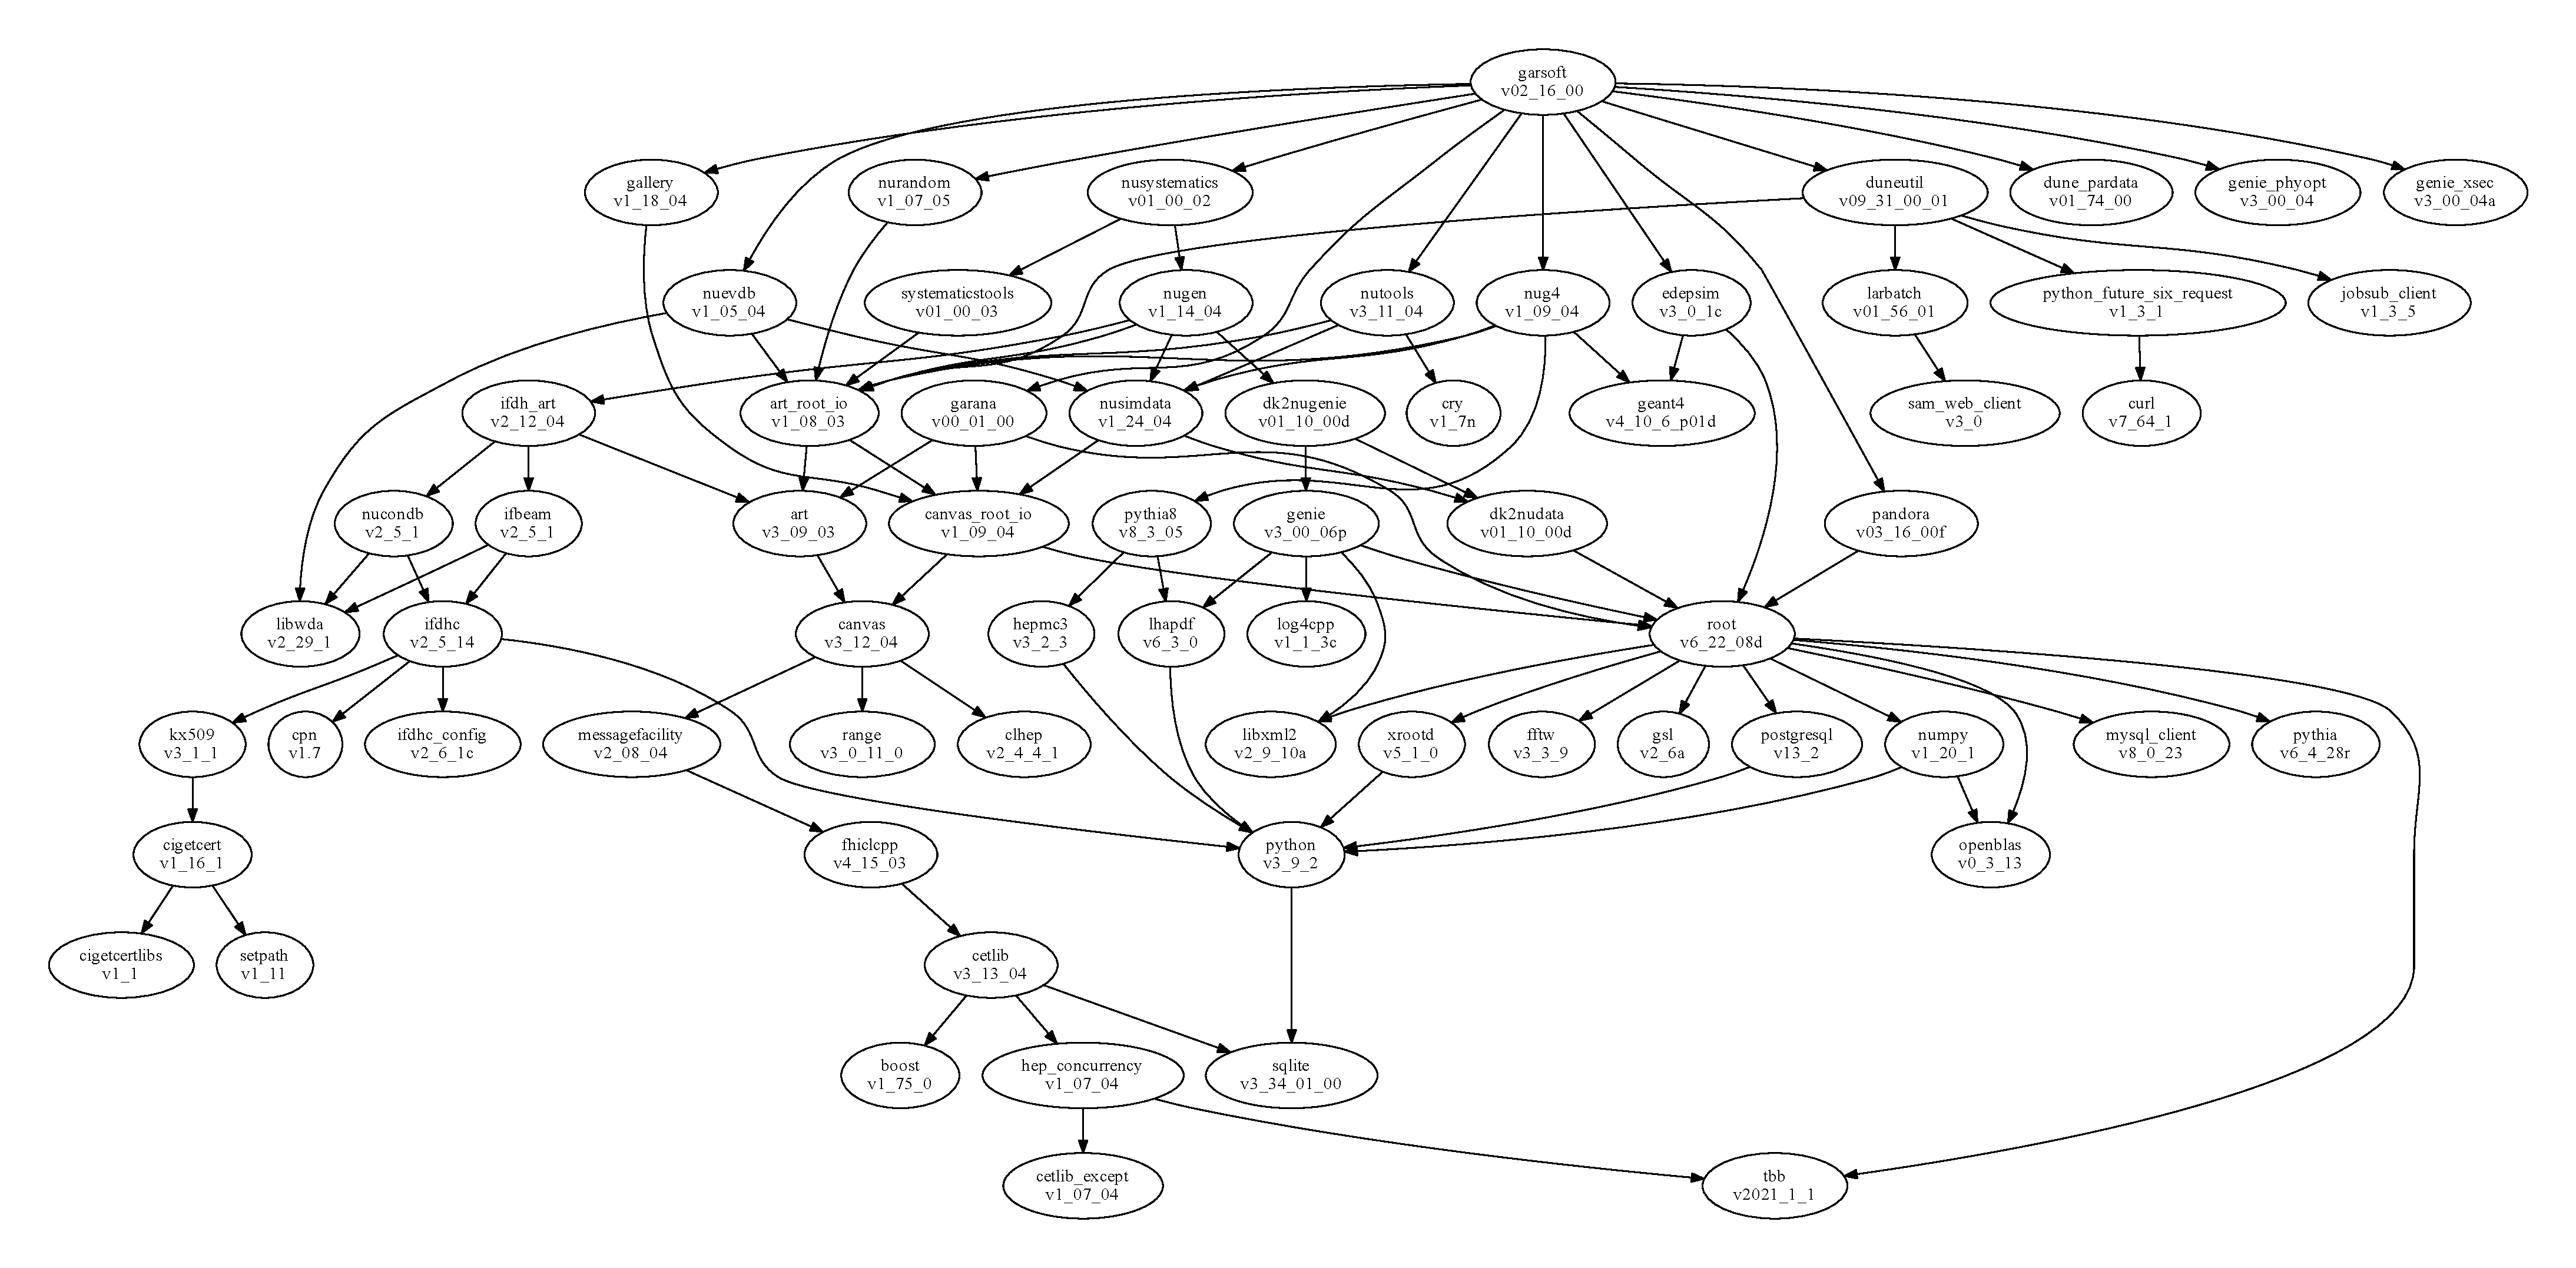
\includegraphics[width=\textwidth]{graphics/CodeManagementFigures/garsoft_v02_16_00_graph.pdf}
\end{dunefigure}

\subsection{SAND Code Management}
\label{sec:codemgmt:sand}

Currently the SAND code, ND-SAND-FastReco, is hosted in GitHub. This code handle the basic reconstruction and detector response mock-up. The full reconstruction and detector response code is currently under private development, but will be made available this spring prior to production integration.  

\subsection{Near Detector Common and Production Tools}
\label{sec:codemgmt:ndproduction}

A repository has been set up in GitHub to manage files that are needed for \dword{nd} production.  These include production scripts, detector geometry descriptions and flux specifications.  It is versioned and installed in \dword{cvmfs} like other DUNE repositories, so that production workflows can be reproduced at later dates. Additionally, common ND geometry code is stored in GitHub, dunendggd.

\section{Continuous Integration \hideme{Junk - draft}}
\label{sec:codemgmt:ci}

The stability of the performance of a large base of shared software requires attention to each change that is committed.  Software releases require validation and approval before being used in analyses intended for publication.  The rapid pace of software development early in the life cycle of the experiment, as well as increased activity as data are first collected and conferences come up, requires constant vigilance to ensure that bugs are not introduced and that software remains backwards-compatible.

To meet this requirement, an automated continuous integration (\dword{ci}) system is currently in operation for the \dword{larsoft}-based code base.  Similar systems, even using the same infrastructure, will be deployed for the \dword{nd} and beam simulations system.  The \dword{ci} system consists of a set of servers that monitor  commits pushed to the central code repositories.  On each commit,   a suitable delay of approximately 15 minutes allows aggregation of commits. % to aggregate commits. 
%each commit pushed to the central code repositories, with a suitable delay of approximately 15 minutes in order to aggregate commits. 
The \dword{ci} system can also be triggered by user interaction, via an authenticated request.  Once triggered, the \dword{ci} system  compiles the changed code as well as any dependencies that are required.  Currently, the \dword{ci} system builds \dword{larsoft} and all experiment code from the head of the develop branch in the repositories. 

The status of the build is stored in a logfile and summarized on a web page.  If a commit causes the build to fail, software managers and the person who committed and/or pushed the commit are notified and the commit is blocked from being merged into the head of develop.  \dword{larsoft} currently implements a pull-request model, in which experiment-appointed Level-2 managers comment on and sign off on changes to the central code, and Level-1 managers perform the actual merging.  A proposed change will not even be sent out for approval unless the \dword{ci} system can build it and validation tests are run to compare output that ought not to have been changed by the new code.

This second step, physics performance validation, requires a more lengthy run through both unit tests and integration tests that run simulation and reconstruction workflows.  These tests run on standard input files and have their random number seeds fixed to constants.  The outputs are compared with reference histograms and a web page summarizes the comparison of the output logfiles, histograms, as well as run times and memory consumption, all of which are available on a web site that monitors these tests.  History plots of variables such as run time and memory consumption are made available on the monitoring web site so that investigations of when the memory usage of a job jumped up can be done without laboriously checking out, building, and running the software in the suspected 
timeframe of interest to find  a particular change.
\end{document}
